\documentclass{article}
\usepackage[utf8]{inputenc}
%\usepackage[german]{babel}
\usepackage{amsmath, amssymb}
\usepackage{amsthm}
\usepackage{graphicx}
\graphicspath{ {images/} }
\newtheorem{theorem}{Satz} %TODO: change counter
\newtheorem{definition}{Definition}
\newtheorem{lemma}{Lemma}
\theoremstyle{plain}
\newcommand{\thistheoremname}{}
\newtheorem{genericthm}[theorem]{\thistheoremname}
\newenvironment{namedthm}[1]
  {\renewcommand{\thistheoremname}{#1}
   \begin{genericthm}}
  {\end{genericthm}}
%\addto\captionsgerman{\renewcommand{\figurename}{Abbildung}}
\renewcommand{\figurename}{Abbildung}
\renewcommand{\proofname}{Beweis}
\renewcommand{\contentsname}{}
\renewcommand\refname{Literatur}

\title{Graphentheorie}
\author{Franziska Butter}
\date{September 2022}

\begin{document}

\maketitle

\section{Übersicht}
	\tableofcontents

\newpage

\section{Was sind Graphen? - Eine Einführung}
In diesem Paper möchte ich eine erste Einführung zum Thema Graphentheorie geben. Wer noch nie mit dem Thema in Berührung gekommen ist, soll nach dem Studieren dieser Einführung einen grundlegenden Überblick über die Basics bekommen. Hierzu beginnen wir mit den gundlegenden Definitionen, werden uns einsteigende Beispiele anschauen, sowie ein paar erste Sätze.\\
\bigskip
\begin{definition} 
            Ein \textbf{Graph} \( G = (V, E)\) besteht aus einer nichtleeren Menge V und einer (möglicherweise leeren) Kantenmenge \(E\), wobei jede Kante \(e \in E\) zwei Knoten \(u, v\) miteinander verbindet.\cite[S.~11]{bue_1}
\end{definition}
\bigskip
Beginnen wir also direkt mit dieser Definition. Zunächst abstrakt wirkend, schauen wir uns doch erst einmal ein Beispiel an:\\
Angenommen, Katrin, Tom, Erik und Lisa sind vier Studierende. Katrin kennt Tom, Lisa und Erik, Lisa kennt Tom und Katrin, Tom kennt Lisa und Katrin, und Erik kennt Katrin. Zusätzlich kennt jeder natürlich noch sich selbst.\\
Diese Freundschaften kann man nun in einem mathematischen Graphen betrachten. Jeder Studierende ist hierbei ein Knoten \(v\) , und jede Freundschaft zwischen zwei Knoten bildet eine Kante \(e\). Zusammen bilden alle Knoten die Knotenmenge \(V\), und alle Kanten die Kantenmenge \(E\).\\
Zusammen bilden \((V, E)\) den Graphen \(G\), welchen man graphisch darstellen kann.\\
\bigskip
\begin{figure}[!htp]
    \centering
    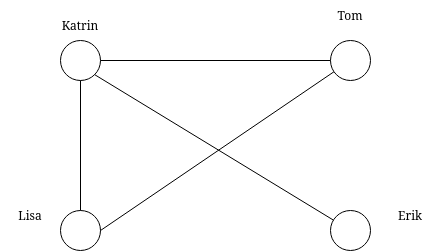
\includegraphics[width=8cm]{vortrag_schriftlich/images/graph_one.drawio.png}
    \caption{Katrin, Lisa, Tom und Erik kennen sich untereinander. Aber: Nicht jeder kennt jeden!}
    \label{fig:fig1}
\end{figure}
\newpage
Nun könne die Knoten und Kanten jeweils verschiedene Beziehungen zueinander haben.\\
Um auf unser Beispiel zurückzukommen: Eine triviale, jedoch erwähnenswerte Erscheinung ist noch, dass jeder sich selbst kennt. Übersetzt in die Sprache der Graphentheorie bedeutet dies, dass eine Kante den gleichen Endpunkt hat. Dieses Phänomen nennt man \textbf{Schlinge}.
\bigskip
Wenn man (redundanterweise) die Information "Tom kennt Lisa und Lisa kennt Tom" angeben möchte, könnte man auch vom Knoten "Tom" eine Kante zum Knoten "Lisa" ziehen, und vom Knoten "Lisa" eine Kante zum Knoten "Tom". Wenn also zwei Kanten den gleichen Endpunkt haben, so nennt man diese \textit{parallel}.\\
\bigskip
Diese Begriffe nochmal in Definitionen zusammengepackt:\\
\begin{itemize}
	\item Wenn \(u = v\) für eine Kante \(e = \{u, v\}\) gilt, so heißt diese Kante \textit{Schlinge}.
	\item Wenn für zwei Kanten \(e, f \in E\) gilt: \(e = f = \{u, v\}\) (gleiche Endknoten), so heißen diese \textit{parallel}. 
	\item Ein Graph heißt \textit{einfach}, genau dann, wenn er weder Schlingen noch parallele Kanten enthält.\cite{bue_1}
\end{itemize}
\begin{figure}[!htp]
    \centering
    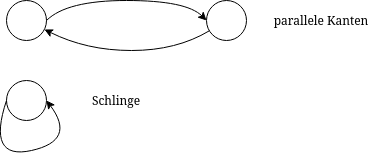
\includegraphics[width=8cm]{vortrag_schriftlich/images/graph_two.drawio.png}
    \caption{Schlingen und parallele Kanten.}
    \label{fig:fig2}
\end{figure}
Unser Beispielgraph mit den Studierenden, welche untereinander befreundet sind, ist hier einfach, da die Informationen, welche Schlingen und parallele Kanten bilden würden, hier redundant, beziehungsweise nicht notwendig sind.\\

\newpage
Nun wird es zunächst wieder etwas technischer. Kanten und Knoten untereinander können auf drei verschiedene Arten und Weisen miteinander in Beziehung stehen. Schauen wir uns diese an:\\
\begin{definition}
    Sei \(G = (V, E)\) ein Graph, \(u, v \in V\) und \(e \in E\).
    Es gilt jeweils:
    \begin{itemize}
        \item \textbf{inzident}:
            Ein Knoten \(v\) und eine Kante \(e\) \textit{inzidieren} miteinander, wenn \(v\) ein \textit{Endknoten} von \(e\) ist.
        \item \textbf{Nachbar eines Knotens}:
            Gilt für eine Menge an Knoten \(\{u, v\} \in E\), so sind \(u\) und \(v\) \textit{adjazent} bzw. \textit{benachbart} in \(G\) und heißen \textit{Nachbarn}.
        \item \textbf{Nachbar einer Kante}:
            Zwei Kanten \(e = \{u, v\} \in E\) und \(f = \{v, w\} \in E\) heißen \textit{adjazent/benachbart}, wenn sie einen gemeinsamen Knoten haben.
    \end{itemize}
\end{definition}
\bigskip
\emph{Frage an den geneigten Leser.} Finde ein Beispiel für einen unendlichen Graphen.
\bigskip
Diese Definitionen macht man sich am Besten klar, indem man sich selbst einmal einen Graphen anschaut (dafür eignet sich beispielsweise unser einführendes Beispiel mit den Studierenden).\\
%%%%TODO: Bild einfügen + überarbeiten!
\subsection{Konventionen}
Bevor wir uns weiter in der Welt der Graphentheorie hervortasten, zunächst ein paar Konventionen, die wir festlegen:
\begin{itemize}
        \item Wir bezeichnen eine  Kante \(e\) hier mit \(e:= \{u, v\}\). Es gibt auch noch Alternativbezeichnungen für Kanten. Was wir NICHT verwenden: \(e = (u, v)\) , \(e = uv\).
        \item \textit{Endknoten.} Wir bezeichnen einen Endknoten einer Kante \(e\) als ein Knoten \(u \in V\), der in einer Kante \(e = \{u, v\}\) enthalten ist. 
        \item Knotenanzahl in einem Graphen: \(n\)
        \item Kantenanzahl in einem Graphen: \(m\)
        \item Wir beschäftigen uns von nun an mit \textit{einfachen} Graphen.
    \end{itemize}

\newpage
\section{Gimme five! (Handshaking-Lemma)}
Nun, da die nötigen Grundlagen gelegt sind, kann es auch schon mit der ersten wichtigen Erkenntnis in der Graphentheorie, nämlich dem Handshaking-Lemma, weitergehen.\\
\bigskip
Bevor wir jedoch dazu kommen, müssen wir erneut eine relevante Definition einführen:\\
\bigskip
\begin{definition} Sei \(G = (V, E)\) ein Graph. Der \textbf{Grad} \(d(v)\) eines Knotens \(v \in V\) ist die Anzahl des Auftretens von \(v\) als Endknoten einer Kante. Wenn \(G\) einfach ist, so ist \(d(v)\) gleich der Anzahl der Nachbarn von v.
\end{definition}
\bigskip
Diese Definition lässt sich sehr einfach auf unseren Beispielgraphen vom Anfang übertragen: Um beispielsweise den Grad des Knotens "Katrin" zu bestimmen, zählen wir einfach, wie viele Kanten von dem Knoten ausgehen, also, mit wie vielen Studierenden Katrin aus der Gruppe von 4 Menschen befreundet ist, also die Anzahl der Nachbarn des Knoten "Katrin". In diesem Falle sind es \(3\) Kanten, also ist Katrin mit 3 Studierenden (Tom, Erik, Lisa) befreundet.\\
Das Zählen der Freunde funktioniert aber nur, da G einfach ist. Würde es beispielsweise noch eine Schlinge für "Studierender x kennt sich selbst" geben, so wäre der Knotengrad jeweils die Anzahl der Nachbarn der Knoten \(+1\).\\
\bigskip
Weiterhin bezeichnen wir für einen Knoten \(v \in V\):
\begin{itemize}
	\item \(\delta(G)\) als \textit{Minimalgrad} eines Graphen, und
	\item \(\Delta(G)\) als \textit{Maximalgrad} eines Graphen.
\end{itemize}
\textit{Frage an den geneigten Leser.}\\
Was sind jeweils der Minimal- und Maximalgrad des Beispielgraphen?\\
\bigskip
Nun können wir auch schon zur versprochenen wichtigen Erkenntnis kommen: Dem Handshaking-Lemma.\\
\begin{namedthm}{Lemma}[Handshaking-Lemma]
Die Summe der Knotengrade entspricht zweimal der Anzahl der Knoten, also
\begin{equation*}
	\sum_{v \in V}d(v) = 2 \cdot |E| = 2m.
\end{equation*}
\end{namedthm}
\bigskip
\begin{proof}
	Um das Handshaking-Lemma zu beweisen, nehmen wir uns einen endlichen einfachen Graphen und zählen die inzidierenden Paare $(v, e)$ auf jeweils zwei verschiedene Arten und Weisen, um beide Seiten der Gleichung zu erhalten.\\
	Schauen wir uns zunächst die linke Seite der Gleichung, also $\sum_{v \in V}d(v)$ an. Die Knotengrade $deg(v)$ bilden die Anzahl der Kanten, mit denen die Knoten $v$ jeweils inzidieren. Um sich dies besser zu verdeutlichen, schauen wir uns einmal unseren Beispielgraphen vom Anfang an, jedoch mit der Veränderung, dass Katrin, Tom, Erik und Lisa sich diesmal zu viert verabreden, um sich alle untereinander kennenzulernen. In Falle eines solchen Treffens würden alle vier sich zu Beginn die Hand untereinander geben. Wenn man die Handschläge in einem Graphen darstellen möchte, dann wäre jeder Knoten mit jedem anderen Knoten durch eine Kante verbunden ($deg(v)$ wäre hier also für alle $v$ $3$: jeder Knoten inzidiert jeweils mit $3$ Kanten). Damit zählt $\sum_{v \in V}deg(v)$ also die inzidierenden Paare $(v, e)$ für alle $v$ im Graphen.\\
	Nun zur linken Seite der Gleichung, also $2 \cdot |E|$. Diese erhält man ganz einfach, indem man sich überlegt, dass jede Kante im Graphen zu genau zwei inzidierenden Paaren gehört, also zu zwei unterschiedlichen Knoten $v_1, v_2$. Dadurch erhält man für jede Kante $e$ des Graphen jeweils die inzidierenden Paare $(v_1, e)$ und $(v_2, e)$. Verdeutlicht am Beispiel bedeutet dies: Zu jedem Handschlag $(e)$ gehören zwei Leute $(v_1, v_2)$ dazu. Also erhält man damit die linke Seite der Gleichung.\\
	Da nun beide Seiten jeweils die gleiche Menge zählen, nämlich die inzidierenden Paare $(v, e)$, erhält man Gleichheit.
\end{proof}
\bigskip
\begin{figure}[!htp]
    \centering
    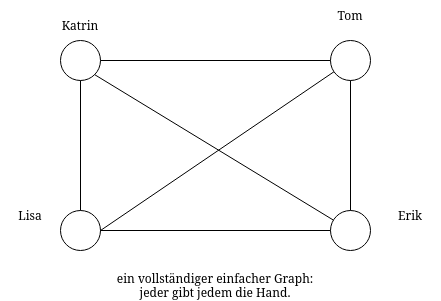
\includegraphics[width=8cm]{vortrag_schriftlich/images/three_h_lemma.drawio.png}
    \caption{Die  Studierenden treffen sich allesamt: Jeder gibt jedem die Hand.}
    \label{fig:fig3}
\end{figure}
\newpage
Aus dem doch recht anschaulichen Handshaking-Lemma können wir als nächstes eine Erkenntnis folgern:\\
\begin{namedthm}{Lemma}
	In einem Graphen ist die Anzahl der Knoten mit \emph{ungeradem Grad} gerade.\\
\end{namedthm}
\bigskip
Dies mag zunächst etwas technisch wirken, ist jedoch ebenfalls recht einfach zu beweisen:
\begin{proof}
	Die Beweisidee hier ist, die Summe auf der linken Seite des Handshaking-Lemma aufzuspalten:\\
	Aus $\sum_{v \in V}d(v) = 2 \cdot |E|$ können wir zunächst folgern, dass die Summe aller Knotengrade immer eine gerade Zahl sein muss.Sei $V$ die Knotenmenge. Nun teilen wir diese in zwei Teilmengen auf:
		\begin{itemize}
			\item{$V_1$:= Die Menge aller Knoten mit ungeradem Knotengrad.}
			\item{$V_2$:= Die Menge aller Knoten mit geradem Knotengrad.}
		\end{itemize}
	Nun können wir folgende Umformung machen:
		\begin{align*}
			&2\text{m} = \sum_{v \in V}d(v) = \sum_{v \in V_1} + \sum{v \in V_2}d(v)\\
			&\Leftrightarrow \underbrace{2m - \sum_{v \in V_2}d(v)}_{\text{gerade}} = \sum_{v \in V_1}\underbrace{d(v)}_{\text{ungerade, da in $V_1$}}\\
		\end{align*}
	Die linke Seite der Gleichung ist offensichtlich gerade. Nicht so ganz trivial zu sehen ist, warum die rechte Seite der Summe ebenfalls gerade sein sollte: Dies muss der Fall sein, da sonst die Gleichung nicht erfüllt werden könnte. Eine Summe von ungeraden Summanden muss zwingend gerade sein, da sonst die linke Seite ebenfalls nicht gerade wäre. Es muss eine gerade Anzahl ovn ungeraden Summanden aufsummiert werden, damit eine Summe gerade wird. Somit ist $|V_1|$ gerade.
\end{proof}
\newpage
\section{Jeder kennt jeden -- vollständige Graphen}
Jetzt, mit etwas Grundwissen ausgestattet, können wir uns einer sehr wichtigen Klasse an Graphen widmen: den \emph{vollständigen Graphen}.\\
\begin{definition}
	Ein Graph $G = (V, E)$ heißt \textbf{vollständig}, wenn jeder Knoten zu jedem anderen benachbart ist.
	\begin{itemize}
		\item[$\rightarrow$] Da $G$ nur von $n$ abhängt, bezeichnen wir $G$ als $K_n$.
		\item[$\rightarrow$] Eine offensichtliche Folgerung daraus ist: $\delta(G) = \Delta(G)$.
	\end{itemize}
\end{definition}
\bigskip
Diese Definition lässt sich leicht veranschaulichen: Im Beispielgraphen vom Anfang erkennt man, dass dies kein vollständiger Graph ist, da sich die vier Studierenden nicht alle untereinander kennen. Ändert man das Beispiel jedoch so ab, wie es beim Beweis des Handshaking-Lemmas getan wurde, erhält man einen vollständigen Graphen: Jeder gibt jedem die Hand, jeder lernt die anderen aus der Gruppe kennen; jeder Knoten ist zu jedem anderen benachbart.\\
\bigskip
\emph{Frage an den geneigten Leser.} Folgere aus dem Handshaking-Lemma: Was ist die Anzahl an Kanten in einem (endlichen) vollständigen Graphen? Warum ist das so?\footnote[1]{Den Beweis hierzu gibt's am Ende des Papers.}\\
\bigskip
In diesem Zusammenhang können wir nun einen weiteren Begriff aus dem Reich der vollständigen Graphen kennenlernen -- nämlich \emph{bipartite Graphen}.\\
\begin{definition}
	Ein Graph $G = (V, E)$ heißt \textbf{bipartit}, wenn seine Knoten in zwei Teilmengen an Knoten $A, B \in V$ so zerlegt werden können, dass nur Kanten \textbf{zwischen}, aber nicht \textbf{innerhalb} einer Knotenmenge verlaufen. Anders gesagt bedeutet das also: In einer jeweiligen Teilmenge $A, B$ existieren keine zueinander benachbarten Knoten.
	\begin{itemize}
		\item[$\rightarrow$] Falls ein Graph die \emph{maximale Anzahl an Kanten} $m_{\mathrm{max}} = |A| \cdot |B|$ besitzt, nennt man ihn \textbf{vollständig bipartit}.
	\end{itemize}
\end{definition}
\newpage
Um zu verdeutlichen, wie ein bipartiter Graph aussieht, hier folgendes Beispiel:
\begin{figure}[!htp]
    \centering
    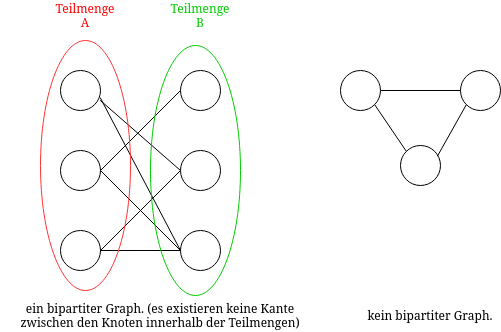
\includegraphics[width=10cm]{vortrag_schriftlich/images/bipartit.drawio.png}
    \caption{Beispiel für einen bipartiten Graphen und einen nicht-bipartiten Graohen.}
    \label{fig:fig4}
\end{figure}
\clearpage
Schauen wir uns zu bipartiten Graphen einmal ein wichtiges Beispiel aus der Graphentheorie an: Den Würfelgraphen:\\
\begin{figure}[!htp]
    \centering
    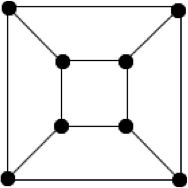
\includegraphics[width=7cm]{vortrag_schriftlich/images/wuerfelgraph.png}
    \caption{Der Würfelgraph.}
    \label{fig:fig5}
\end{figure}\cite{website:wikiversity}
\newpage
\section{Was sind Wege?}
Was sind Wege? - eine einfache Frage, würde man sich vielleicht denken, jedoch sind mathematische Wege etwas anderes als das, was wir umgangssprachlich als "Weg" bezeichnen. Bevor wir diese Frage sauber mathematisch beantworten können, müssen wir jedoch zunächst noch etwas Vorarbeit leisten - beginnend mit Teilgraphen:\\
\begin{definition}
	Sei $G = (V, E)$ ein Graph. Ein Graph $G' = (V', E')$ ist ein \textbf{Teilgraph} von $G$, wenn $V' \subseteq V$ und $E' \subseteq E$ gilt.
		\par\bigskip
	Falls $E'$ jede Kante aus $E$ enthält, die zwei Knoten aus $V'$ verbindet, so sagt man: $G'$ ist ein von $V' \subseteq V$ \textbf{induzierter Teilgraph} bzw.\ \textbf{Untergraph} von $G$.
\end{definition}
Um diese Definitionen besser nachvollziehen zu können, hierzu einmal ein paar Beispiele:\\
\vfill
\begin{figure}[!htp]
    \centering
    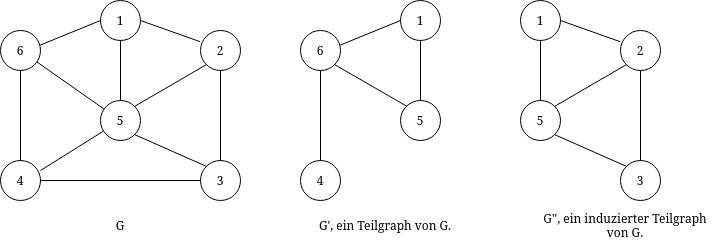
\includegraphics[width=10cm]{vortrag_schriftlich/images/teilgraph.drawio.png}
    \caption{Ein Teilgraph und ein induzierter Graph.}
    \label{fig:fig6}
\end{figure}
\vfill
Nun kommen wir zur nächsten Definition, welche wir ebenfalls noch als Vorarbeit benötigen, um schließlich den Begriff des Weges -- eine weitere sehr Wichtige Klasse an Teilgraphen -- einzuführen:\\
\begin{definition}
	Ein \textbf{Kantenzug $Z$} in $G$ ist eine Folge von Knoten und Kanten in $G$, die sich wie folgt hintereinanderschreiben lässt:
	 \begin{equation*}
		Z = e_0e_1e_2 \ldots e_k
	\end{equation*}
	 wobei $e_i = \{x_i, x_{i+1}\}$ gilt ($x_i \in V$ sind hier die Knoten).
\end{definition}
\bigskip
Ein Kantenzug ist also genau das, wonach es klingt - man schreibt einfach verschiedene "benachbarte" Kanten hintereinander auf. Dabei ist es wichtig zu erwähnen, dass hierbei gleiche Kanten mehrfach durchlaufen werden dürfen, und Start- und Endknoten eines Kantenzuges sind egal.\\
\begin{small}
	\begin{emph}
		Es ist anzumerken, dass der Kantenzug alternativ auch noch so definiert werden kann:\\
		\begin{equation*}
			Z = x_0e_0x_1e_1x_2e_2 \ldots x_{k-1}e_{k-1}x_k
		\end{equation*}
		wobei $e_i = \{x_1, x_{i+1}\}$ gilt. (Die Definition läuft also über die Knoten anstatt die Kanten.)
	\end{emph}
\end{small}
\bigskip
Nun sind wir soweit, dass wir endlich einen mathematischen Weg definieren können:\\
\begin{definition}
	Sei $Z$ ein Kantenzug. Definiere nun $Z$ als
	\begin{itemize}
		\item einen \textbf{Weg}: Alle Kanten in $Z$ sind verschieden. Die Knoten $x_0$ und $x_k$ sind die \emph{Endknoten} eines Weges $p$.
		\item einen \textbf{Kreis}: Ein \textbf{Kreis} ist ein Weg, bei dem gilt: $x_0 = x_k$ (gleicher Anfangs- und Endknoten).
	\end{itemize}
\end{definition}
\bigskip
Ein Weg ist also ein Kantenzug, der zwar die gleichen Knoten durchlaufen darf, jedoch keine gleichen Kanten. Bei einem Kreis dürfen ebenfalls gleiche Knoten durchlaufen werden, und Anfangs- und Endknoten müssen zwingend gleich sein, also $x_0 = x_k$.\\
\bigskip
Aus dieser Definition folgt sofort:
\begin{definition}
	Die \textbf{Länge} eines Weges ist die Anzahl der Kanten im Kantenzug, der den Weg definiert.
\end{definition}
\bigskip
%%%TODO: Ist das richtig?
%%%\emph{Frage an den geneigten Leser.}\\
%%%In welcher Art von (endlichen) Graphen lässt sich immer ein Kreis finden?\\
\vfill
\begin{figure}[!htp]
    \centering
    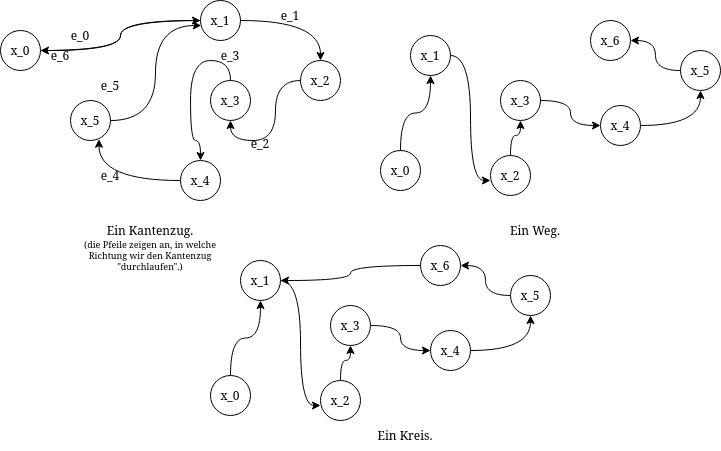
\includegraphics[width=10cm]{vortrag_schriftlich/images/kantenzug_weg.drawio.png}
    \caption{Kantenzug, Weg und Kreis.}
    \label{fig:fig7}
\end{figure}
\vfill
\newpage
Nun, da wir um diese wichtigen Definitionen wissen, gibt es noch eine \emph{einfache} Sache zu beachten;\\
\begin{definition}
	Wir definieren...
	\begin{itemize}
		\item \textbf{einfacher Weg:} Ein Weg heißt \emph{einfach}, wenn keine doppelten Knoten vorkommen, also kein Knoten doppelt "`durchlaufen"' wird.
		\item \textbf{einfacher Kreis:} Ein Kreis heißt \emph{einfach}, wenn außer dem Endknoten kein Knoten doppelt vorkommt.
	\end{itemize}
\end{definition}
Kommen wir jetzt zu einer sehr machtvollen Erkenntnis über einfache Wege und einfache Kreise:\\
\begin{theorem}
	Jeder Graph $G$ enthält einen einfachen Weg der Länge $\delta(G)$. \emph{(I.)} Falls $\delta(G) \geq 2$ gilt, dann enthält er auch einen einfachen Kreis von mindestens der Länge $\delta(G) + 1$. ($\delta(G)$ ist der Minimalgrad.) \emph{(II.)}
\end{theorem}
Wollen wir dies nun beweisen.\\
\begin{proof}
	Sei $G = (V, E)$ ein Graph. Wir wollen zunächst Teil (I.), und dann Teil (II.) beweisen.\\
	\emph{Teil (I.)} Sei $G' = (V', E')$ ein Teilgraph von G, der jeweils die Knoten und Kanten mit $\delta(G)$ enthält. Wenn $\delta(G) = 1$ gilt, dann ist klar, dass unsere Aussage wahr ist: Dann besteht unser Teilgraph $G'$ nämlich nur aus zwei Knoten und einer Kante, und unser Weg $p$ lautet $p = ae_0b$, wobei $a, b \in V'$ und $e_0 \in E'$.\\
	Sei nun $p = x_0 \ldots x_k$ ein längster einfacher Weg in $G$. Wir nehmen nun an, dass $x_k$ einen Nachbarn $a$ hat, welcher nicht auf $p$ liegt. Dies bedeutet nun aber, dass $p$ um die Kante $\{x_k, a\}$ verlängert werden muss, sonst wäre $a$ kein Nachbar von $x_k$.\\
	Nun haben wir also einen neuen Weg $\bar{p} = x_0 \ldots x_k a$. Trivialerweise ist $\bar{p}$ ein längerer Weg als $p$, da $\bar{p}$ um eine Kante länger ist.\\
	Dies erschafft jedoch einen Widerspruch dazu, dass $p$ der längste einfache Weg ist, denn nun ist es $bar{p}$.\\
	$\Rightarrow$ Daraus können wir folgern, dass alle Nachbarn von $x_k$ auf $p$ liegen müssen, denn würden sie es nicht, wäre $p$ kein längster einfacher Weg mehr.\\
	$\Rightarrow$ Es gilt: $$k \ge \text{d}(x_k) \geq \delta(G)$$.\\
	\emph{Teil (II.)} Sei nun $x_i$ ein Nachbar von $x_0$, der am weitesten entfernt von $x_0$ liegt. Vorstellen kann man sich diese Konstruktion wie folgt:\\
    \vfill
	\begin{figure}[htp]
	    \centering
	    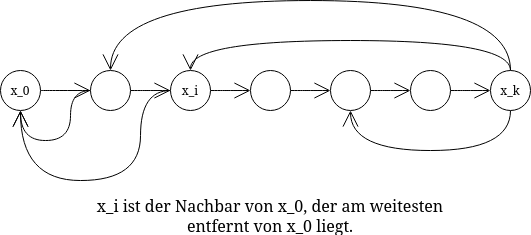
\includegraphics[width=10cm]{vortrag_schriftlich/images/proof_thm.drawio.png}
	    \caption{Ein längster einfacher Weg $p = x_0 \ldots x_i \ldots x_k$}
	    \label{fig:fig8}
	\end{figure}
    \vfill
	Aus Teil \emph{(I.)} folgern wir: Alle Nachbarn von $x_0$ liegen auf $p = x_0 \ldots x_i \ldots x_k$.\\
	$\Rightarrow$ Ein einfacher Weg $p' = x_0 x_1 \ldots x_i$ hat mindestens eine Länge von $\delta(G) \geq 2$.\\
	$\Rightarrow$ Dadurch entsteht auch ein einfacher Kreis $k = x_0 \ldots x_i x_0$ von mindestens der Länge $\delta(G) + 1 \geq 3$, bei dem keine Kante und kein Knoten doppelt durchlaufen werden, womit wir unsere Aussage bewiesen haben.
\end{proof}
Dies gibt uns die mächtige Erkenntnis, dass wir in jedem (endlichen, einfachen) Graphen einen einfachen Weg und in jedem Graphen mit $\delta(G) \geq 2$ sogar einen einfachen Kreis finden können!\\
\bigskip
Zu guter letzt wollen wir uns in diesem Kapitel noch eine Definition anschauen, welche im weiteren Verlauf der Graphentheorie sehr wichtig werden wird: Zusammenhängende Graphen.\\
\begin{definition}
	Ein Graph $G$ heißt \textbf{zusammenhängend}, wenn zu je zwei Knoten $u, v \in V$ von $G$ ein \emph{Weg} von $u$ nach $v$ existiert (mit $u$ als Anfangs- und $v$ als Endknoten).
	\par\bigskip
	Nicht zusammenhängende Graphen heißen \textbf{unzusammenhängend}.
	\par\bigskip
	Eine \textbf{Zusammenhangskomponente} $H$ von $G$ ist ein \emph{maximal zusammenhängender Teilgraph} von $G$.\footnote[2]{Intuitiv bedeutet das also: $H$ ist eine Zusammenhangskomponente genau dann, wenn H selbst zusammenhängend ist, und \emph{kein Weg aus H herausführt},also keine Knoten in H von Wegen außerhalb von H erreichbar sind.}
\end{definition}
Man kann sich zum besseren Verständnis dieser nun doch recht abstrakten Definitionen vorstellen: Zusammenhangskomponenten sind quasi das "Gegenstück" zu bipartiten Graphen \footnote[3]{Ausnahme hierbei bilden isolierte Punkte als Graph.}.
\bigskip
Um sich besser vorstellen zu können, was diese Definitionen eigentlich meinen, hier ein Beispiel:\\
\begin{figure}[!htp]
    \centering
    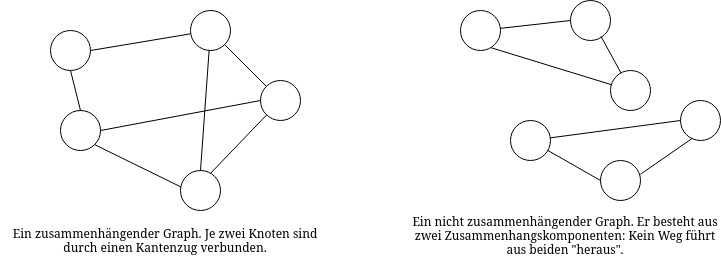
\includegraphics[width=13cm]{vortrag_schriftlich/images/zsmhaengend.drawio.png}
    \caption{Zusammenhängeder Graph und Zusammenhangskomponenten.}
    \label{fig:fig9}
\end{figure}

\newpage
\section[Wozu das Ganze?]{Wozu das Ganze? (Ausblick, Anwendungen)}
\subsection{Ausblick}
Schauen wir uns zuletzt an, wozu wir das Ganze eigentlich benötigen. Wozu Graphentheorie? Was sind die Anwendungen davon? Und welche Themen bauen auf den jetzt geschaffenen Grundlagen auf? Letzteres wollen wir zuerst untersuchen:\\
Folgende Themen werden wir uns im weiteren Verlauf des Seminars anschauen:\\
\begin{itemize}
	\item{Das kürzeste-Wege-Problem: Wie ermitteln Navigationsgeräte den "kürzesten" beziehungsweise "schnellsten"/ $\ldots$ Weg, wenn man irgendwo hinfahren möchte?}
	\item{Rundreisen: Angenommen, ein Reisebüro möchte eine Rundreise erstellen. Die Aufgabe hier lautet, einen Kreis zu finden, der alle Knoten eines Graphen durchläuft, wobei die Knoten hier die angefahrenen Ziele der Rundreise sind, und die Kanten sind die zurückgelegten Strecken.}
	\item{Färbungsproblem: Man möchte Graphen einfärben. Ein gutes Beispiel hierfür wäre der Würfelgraph. Ein weiteres Beispiel wäre, dass ein Lehrer einen Stundenplan erstellen möchte: Die Knoten sind der Dozent mit seinem jeweiligen Kurs, und wenn zwei Knoten durch eine Kante verbunden sind, dürfen zwei Veranstaltungen nicht gleichzeitig stattfinden. Ziel ist nun, alle Knoten mit möglichst wenig Farben einzufärben.}
\end{itemize}

\subsection{Anwendungen}
Die Graphentheorie hat sehr viele Anwendungen im "echten Leben". Dies mag vielleicht im ersten Moment überraschend wirken, jedoch findet man sie an vielen (unerwarteten) Stellen, Ecken und Enden. Vor allem in den Naturwissenschaften sind sie häufig anzutreffen:\\
\begin{itemize}
	\item{Das Internet! Das Internet ist ein einziger riesiger Graph: Die Knoten sind Websites und die Kanten sind Hyperlinks, welche die Websites des Internets miteinander verbinden.}
	\item{Chemie (chemische Graphentheorie): Es existiert eine ganze Sparte in der Chemie, welche die chemische Graphentheorie ist. Molekülverbindungen werden als Graph dargestellt. Hierbei sind die Knoten die Atome eines Stoffes, und die Kanten stellen die Bindungen zwischen den Atomen dar.}
	\item{Äquivalenzreaktionen in der Mathematik. Hierbei sind die Knoten die jeweiligen Elemente, und die Kanten zeigen an, welche zwei Elemente jeweils in Relation zueinander stehen.}
\end{itemize}
Wie wir sehen, sind die Anwendungen der Graphentheorie sehr vielfältig: Wir finden sie fast überall in der Wissenschaft, spezifisch vor allem in der Informatik.\\
\hrule
\bigskip
Dies bringt unseren kleinen Ausflug in die Graphentheorie zu einem Ende. Da die Basics nun gelegt sind, kann man sich nun in die weiteren Tiefen dieses Themengebietes stürzen.
\newpage
\begin{small}
	Die versprochenen Auflösung zu der kleinen Aufgabe gibt's hier:\\
	\begin{proof}
		Wir wollen also die Anzahl an Kanten in $G$ feststellen, falls $G$ ein vollständiger Graph ist.\\
		Dies machen wir mit folgender Überlegung:\\
		Wir wissen, dass in vollständigen Graphen gilt: Der minimalste Knotengrad ist gleich dem maximalsten Knotengrad. Ein vollständiger Graph $G$ hat $n$ Gesamtknoten. Mit diesen Informationen haben wir:\\
		\begin{equation*}
			\underbrace{\sum_{v \in V} \text{d(v)}}_{\text{linke Seite des Handshaking-Lemmas}} = \sum_{v \in V}\Delta(G) = \sum_{v \in V} n - 1 = \sum n \cdot (n - 1) = \underbrace{2m}_{\text{rechte Seite des Handshaking-Lemmas}}.
		\end{equation*}
		Aus diesen Gleichheiten erhält man nun durch einfache Umformung:\\
		$$m = \frac{n(n - 1)}{2}$$
		Und somit haben wir die Gesamtanzahl in einem vollständigen Graphen erhalten und sind fertig.
	\end{proof}
\end{small}
\newpage
\section{Literaturverzeichnis}

\bibliography{vortrag_schriftlich/bibliography}
\bibliographystyle{plain}
\end{document}
